\section{Background}
\label{sec:background}

\subsection{DAT-SPECT for Detecting Parkinson's Disease}
\label{subsec:datspect}

% Parkinsons disease - Reduction in DAT

Dopaminergic (DA) neurons in the substantia nigra pars compacta (SNpc), a region of the human midbrain, 
are of high physiological importance in the regulation of various cognitive mechanisms 
and voluntary movement control in humans~\citep{Luo2016-zj}.
Dopamine transporters (DAT) are proteins located on the presynaptic plasma membrane 
that reuptake dopamine released into the synaptic cleft~\citep{Giros1993-xb}.
Ligands that bind to the DAT protein can inhibit the reuptake mechanism.
Presynaptic DAT ligands labeled with radioactive material are commonly used as radiotracers for nuclear medical imaging,
aiming to assess the integrity of dopaminergic neurons.
Figure~\ref{fig:dat_tracer_synapse} illustrates a dopaminergic synapse, 
highlighting the transporters and receptors to which different radiotracers can bind.

\begin{figure}[ht]
  \centering
  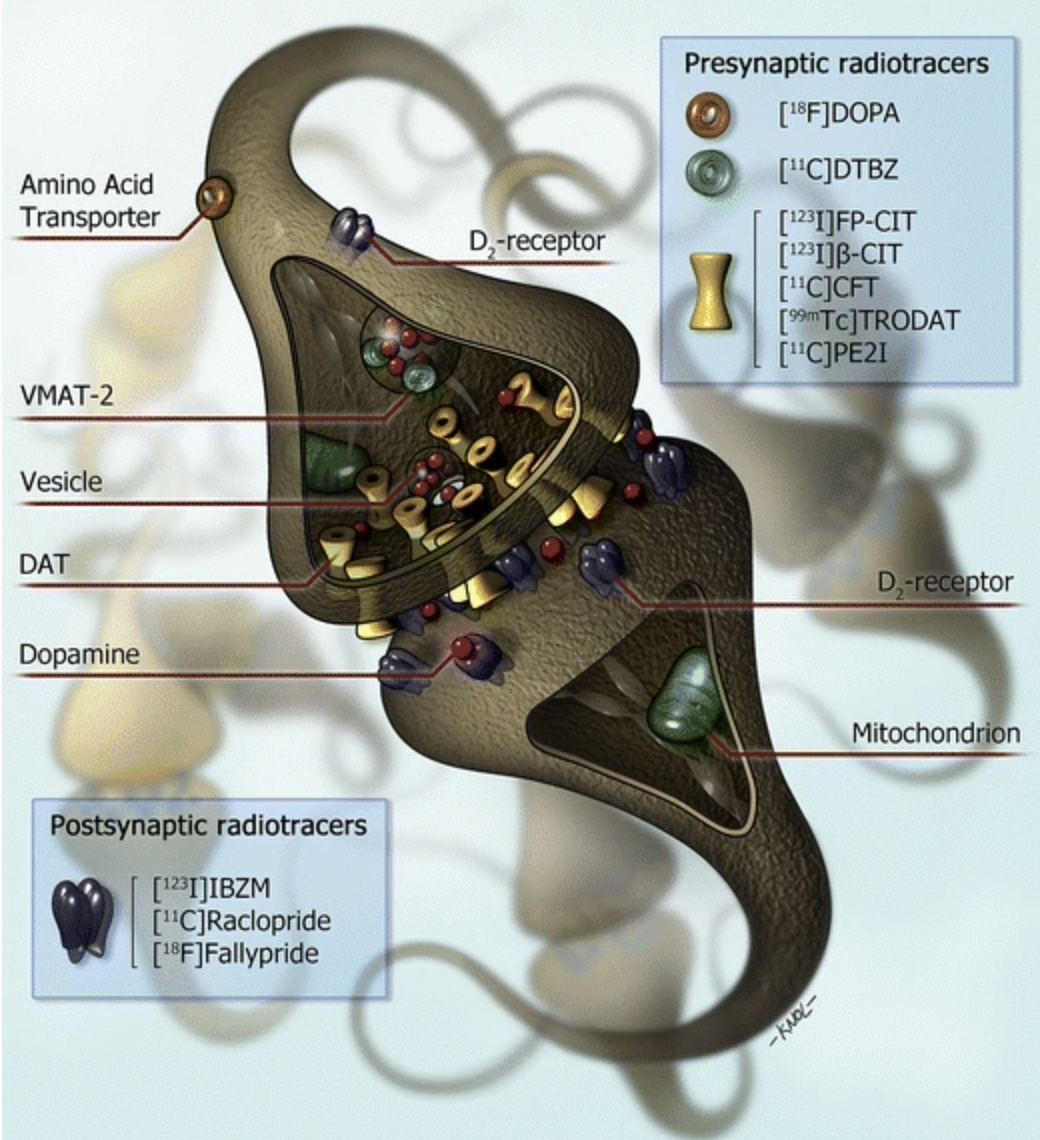
\includegraphics[width=0.7\textwidth]{content/figures/da_synapse.png}
  \caption{Dopaminergic synapse, adopted from~\cite{Booij2008-hh}.
  Postsynaptic radiotracers specifically bind to the $D_2$ dopamine receptor. 
  Presynaptic radiotracers bind to specific dopamine transporters such as Amino Acid Transporter, VMAT-2 or DAT.
  As an example, Ioflupane Iodine-123 ([$^{123}$I]FP-CIT) specifically binds to the dopamine transporter (DAT).} 
  \label{fig:dat_tracer_synapse}
\end{figure}

Parkinson's disease (PD) as well as 'atypical' neurodegenerative Parkinsonian syndromes (PS) 
are both associated with the progressive loss of DA neurons in the SNpc 
that project to the dorsal striatum via the nigrostriatal pathway~\citep{Piggott1999}.
The reduced availability of DAT in the striatum is a well-validated biomarker 
for nigrostriatal degeneration in PD~\citep{Bernheimer1973, Fazio2018, Niznik1991}.
The reduction in striatal DAT availability is significantly advanced even in the earliest symptomatic (motor) stages of PD, 
as the degeneration of dopaminergic nerve endings in the striatum represents 
an early step in the pathological PD cascade~\citep{Bernheimer1973, Fazio2018, Niznik1991}.
The compensatory downregulation of the DAT expression in the remaining nerve endings 
leads to a more pronounced loss of striatal DAT~\citep{Lee2000, Saari2017, Honkanen2019}.
Secondary PS's are typically not associated with nigrostriatal degeneration or the loss of striatal DAT. 

% DAT-SPECT -> what does SPECT measure
The reduction in striatal DAT availability can be detected by Single Photon Emission Computed Tomography (SPECT) 
imaging with DAT ligands~\citep{Kuikka1995, Abi-Dargham1996}.
The radiolabeled DAT ligand Ioflupane Iodine-123 (trade name: $\text{DaTscan}^{\copyright}$), also [$^{123}$I]FP-CIT, 
exhibits a high affinity for presynaptic DAT and 
has been approved as a SPECT tracer in both the US and Europe~\citep{Neumeyer1994}.
Figure~\ref{fig:siemens-healthineers_MI_symbia-evo} illustrates an example of a SPECT scanner.
The DAT-SPECT imaging procedure can be briefly described as follows.
First, the patient is administered with a radiolabeled DAT ligand,
allowing the radiolabeled ligand to bind specifically to the striatal DAT.
The gamma rays emitted from the DAT regions are detected using a rotating (single-head or multiple-head) gamma camera
which captures planar projection (2D) images at multiple angles~\citep{Patton2008-xl}.
The obtained projection images are then filtered and 
backprojected to a 3-dimensional radioactivity distribution SPECT image~\citep{Patton2008-xl}.
The photons emitted from the radiolabeled ligand undergo attenuation and Compton scattering
due to interactions with human tissue which can lead to a distorted radioactivity distribution~\citep{Patton2008-xl}.
To obtain a more accurate representation of the radioactivity distribution, 
attenuation and scatter correction techniques can be applied after the backprojection~\citep{Patton2008-xl}.

\begin{figure}[ht]
  \centering
  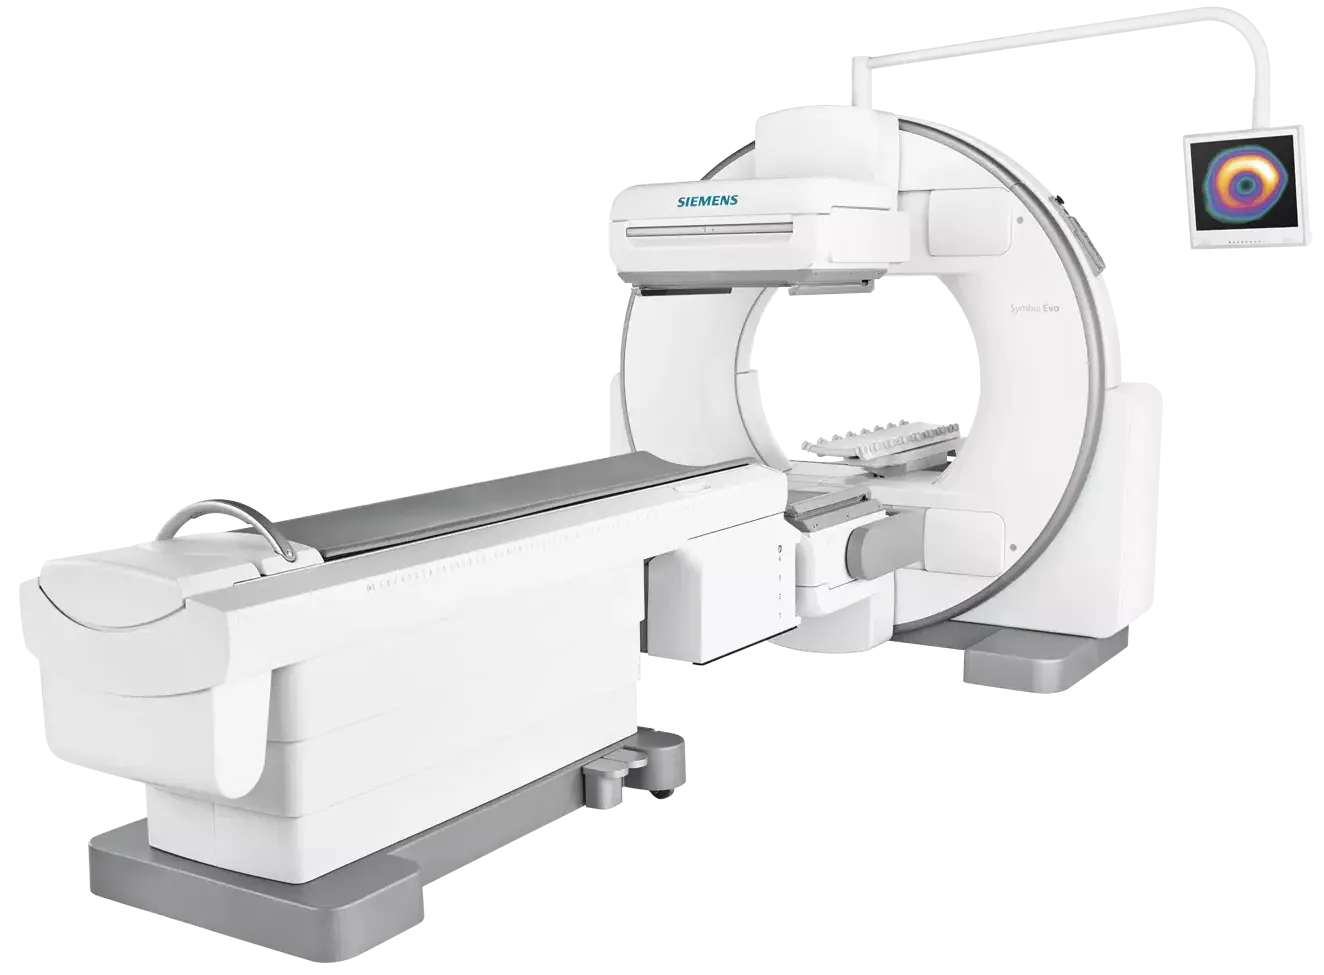
\includegraphics[width=0.85\textwidth]{content/figures/siemens-healthineers_MI_symbia-evo.png}
  \caption{Symbia Evo™ SPECT scanner by Siemens Healthineers. Image source: \cite{SymbiaEvo_siemens}.} 
  \label{fig:siemens-healthineers_MI_symbia-evo}
\end{figure}

A recent review, which involved a non-systematic meta-analysis of DAT-SPECT with [$^{123}$I]FP-CIT in patients with PS, 
confirmed that DAT-SPECT exhibits high sensitivity (median 93\%) and high specificity (median 89\%) 
in differentiating PD from secondary PS in patients with 
clinically uncertain parkinsonian syndrome (CUPS)~\citep{Buchert2019-ya}.
Moreover, the review demonstrated that DAT-SPECT results in a change in diagnosis for about 40\% of patients with CUPS
and leads to a change in treatment for a similar proportion of these patients~\citep{Buchert2019-ya}. 
Thus, DAT-SPECT with [$^{123}$I]FP-CIT is a highly accurate diagnostic method
that significantly influences the diagnosis and treatment of patients with CUPS.
Guidelines from professional neurological societies have therefore strongly emphasized 
the role of DAT-SPECT with [$^{123}$I]FP-CIT in recent years~\citep{Tatsch2013}.
For example, the current version of the S3 guideline “Idiopathic Parkinson syndrome” of the 
German Society of Neurology states that DAT-SPECT \textit{should} be conducted at an early disease stage in CUPS patients.

\subsection{Convolutional Neural Networks for Image Classification}
\label{subsec:randfors}

The rise of Convolutional Neural Networks (CNNs) enabled significant performance breakthroughs 
in various machine learning tasks, including image classification, object detection and semantic segmentation.
Today CNNs are used in medical research to support the diagnosis 
of tumors~\citep{Tiwari2022-wr, Gunashekar2022-rl, Gao2021-zu}, 
cardiovascular diseases~\citep{Yoon2023-ik, Li2022-yn}, 
Alzheimer's disease~\citep{Basaia2019-pg, Folego2020-ak} 
and Parkinson's disease~\citep{Hathaliya2022, Magesh2020, Li2023-ym}
through diverse imaging modalities such as
histopathological images, magnetic resonance imaging (MRI), positron emission tomography (PET) and SPECT.
Continuous research in the explainable AI domain has the potential to enhance the trustworthiness 
of automatic medical diagnosis through explanatory techniques~\citep{Ribeiro2016, Petsiuk2018, Dhurandhar2018, Chaddad2023-zl}.

Convolutional Neural Networks typically consist of many convolution-pooling blocks, 
each with an activation function in between, followed by fully-connected layers that lead to the output layer.
Convolutional layers use a set of filters to extract different local features from the input 
whereas pooling layers are used for the reduction of spatial dimensionality.
The usage of batch normalization layers as a regularization technique can lead to an improved convergence of the model.
The parameters of a CNN are trained using a gradient descent-based algorithm that aims to optimize a specific loss function.
The Adam optimization algorithm~\citep{Diederik2015} allows for fast and smooth convergence 
and is therefore a common choice for optimization.
In a binary classification scenario, the optimization target is the binary cross-entropy loss,
while for multi-class classification the target is the categorical cross-entropy loss.

A challenging effect that occurs in deep neural networks is the vanishing gradient 
as it is backpropagated through the neural network during optimization (vanishing gradient problem).
The residual network (ResNet) architecture~\citep{He2016} was proposed to mitigate the vanishing gradient problem.
In comparison to regular building blocks the ResNet architecture incorporates a residual (skip) connection 
into its building blocks, as demonstrated in Figure~\ref{fig:normal_and_residual_layer}.
The inclusion of the residual connection leads to a larger gradient compared to a scenario where it is absent.
Thereby the residual network architecture allows the training of deeper neural networks.
Also, the residual connection facilitates the learning of the identity function using a shallow model~\citep{He2016}.

\begin{figure}[ht]
  \centering
  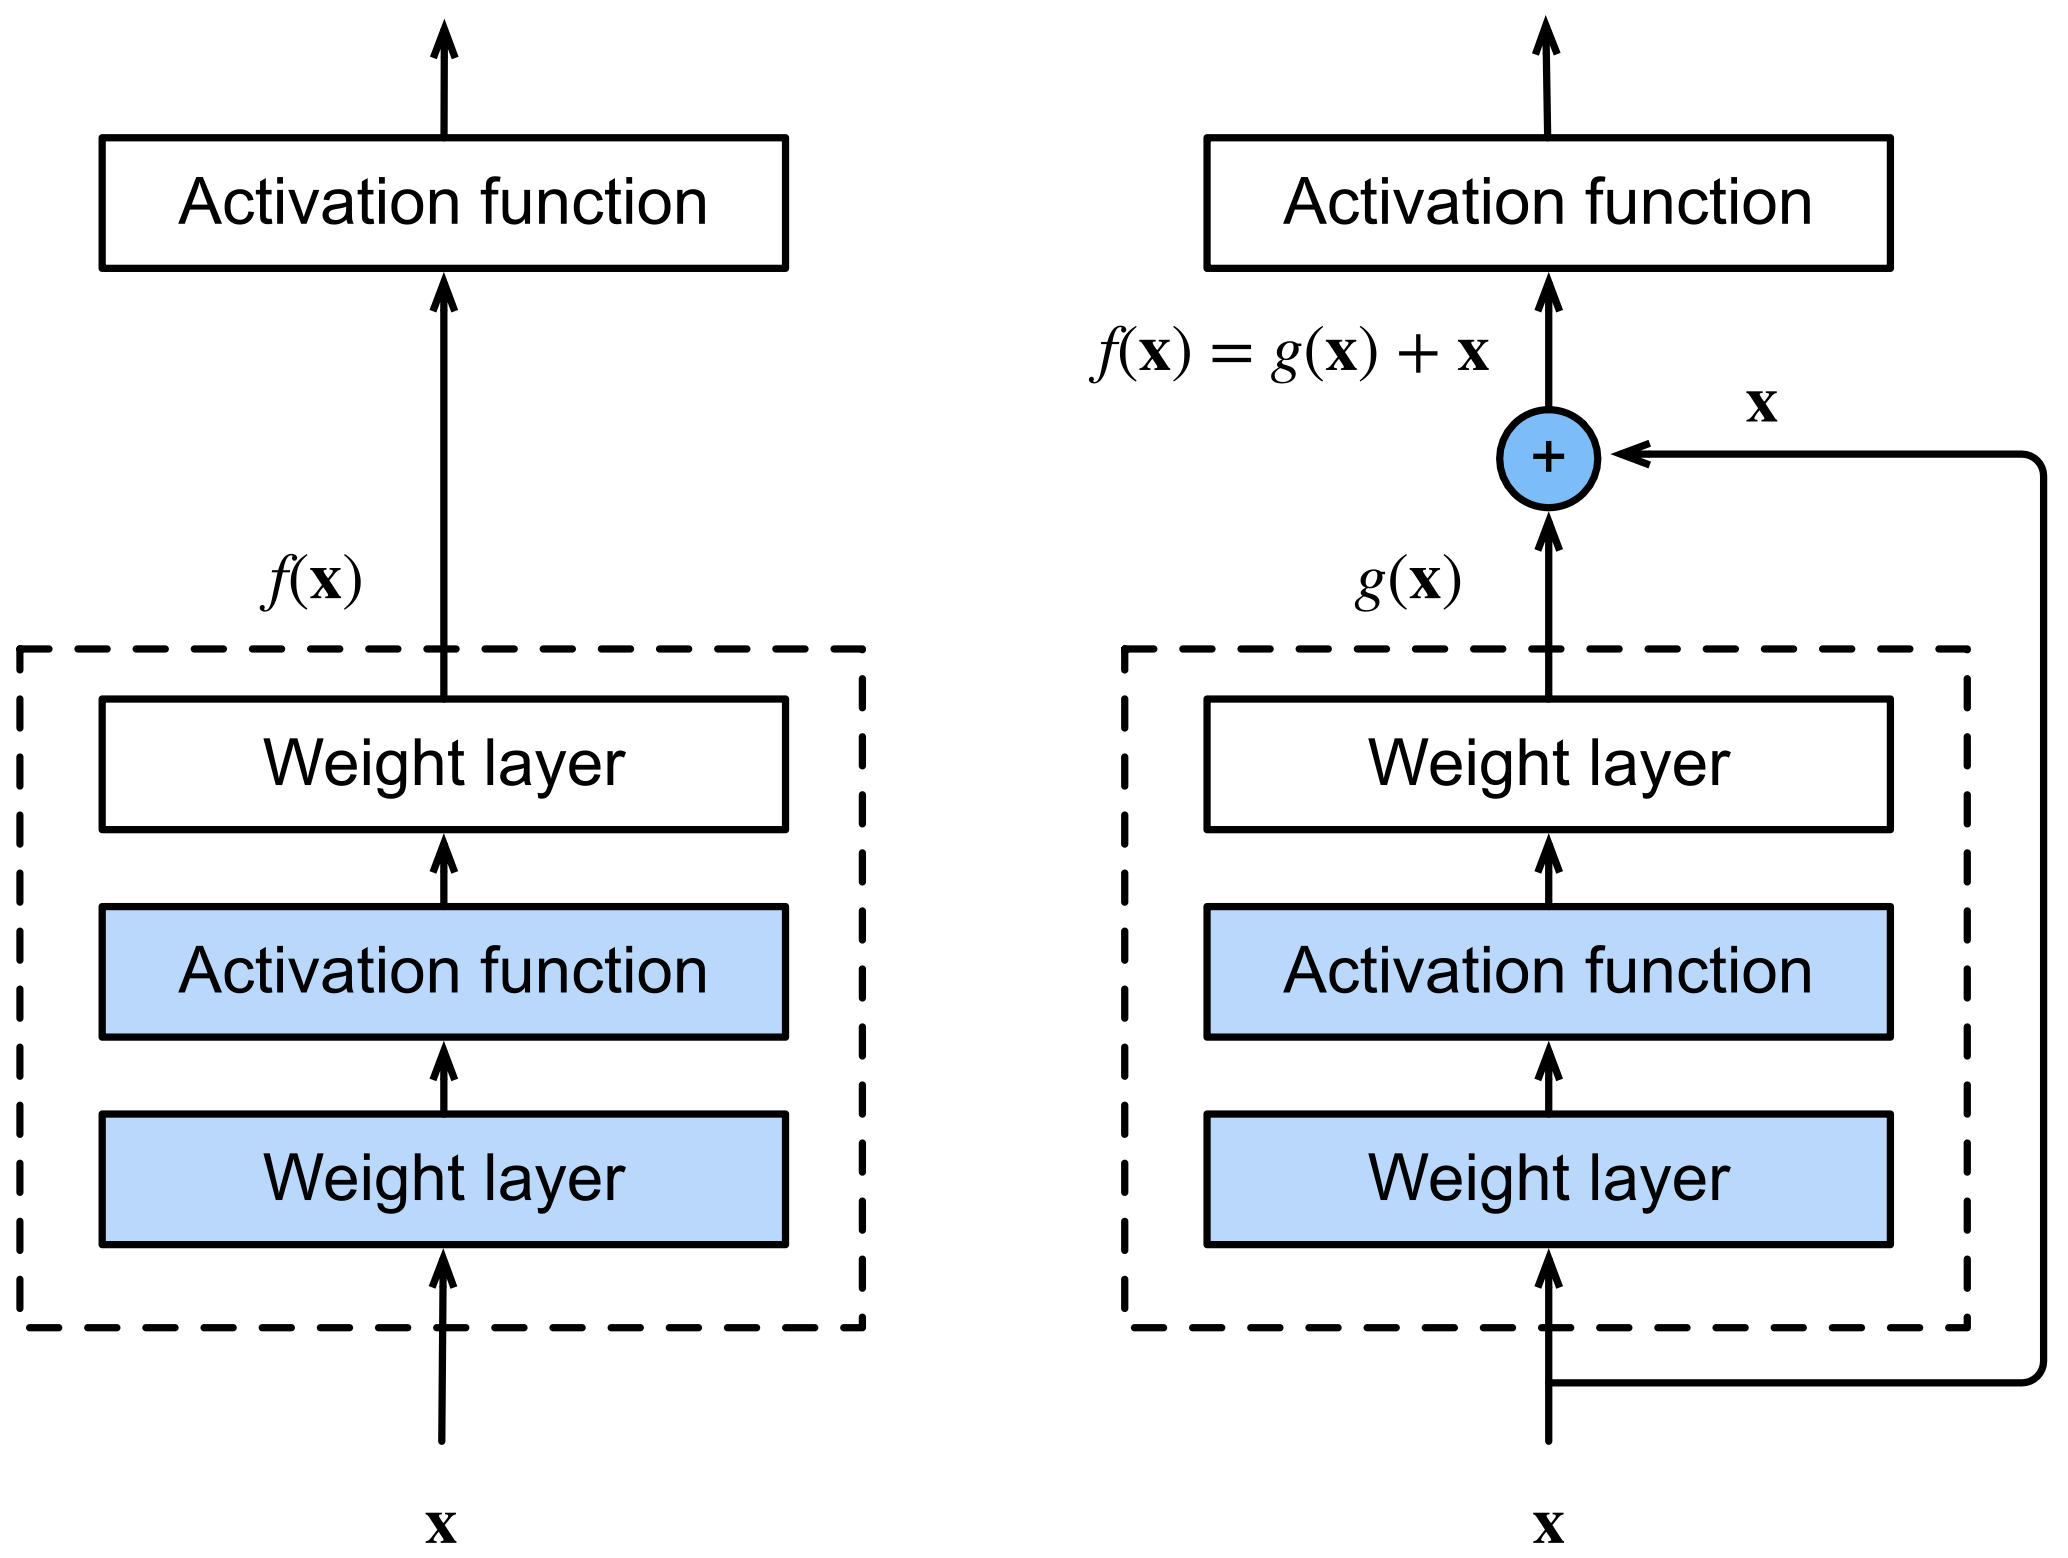
\includegraphics[width=0.85\textwidth]{content/figures/residual_block.png}
  \caption{Residual block (right) in comparison to a regular block (left), adopted from~\cite{Zhang2023}.} 
  \label{fig:normal_and_residual_layer}
\end{figure}


\subsection{Evaluation metrics for Binary Classification}

For the assessment of the classification performance of a binary classification model,
multiple statistical metrics can be used, each focusing on different performance aspects.
Given a set of input features and a decision threshold, 
the binary classification model predicts them as either positive or negative, either correctly or incorrectly.
Thereby the model produces a certain amount of True Positives (TP), True Negatives (TN), False Positives (FP)
and False Negatives (FN), which are then used to calculate the desired metric.

To obtain an overall measure of the classification correctness of the model across all classes
one can calculate the overall accuracy:

\begin{equation}
  \label{eq:acc}
  \text{Accuracy} = \frac{\text{TP + TN}}{\text{TP + TN + FP + FN}} \;.
\end{equation}

The overall accuracy is a suitable metric for balanced datasets with a similar amount of positive and negative cases.
For imbalanced datasets, the overall accuracy provides little informative value 
since it tends to express the accuracy for cases from the majority class.

Sensitivity and specificity are used to gain a more differentiated understanding of the model performance.
In a medical diagnostic scenario, sensitivity, also known as True Positive Rate (TPR),
expresses the ability of the model to correctly classify `disease' (positive) cases~\citep{Parikh2008-ch} 
and can be calculated as

\begin{equation}
  \label{eq:sens}
  \text{Sensitivity} = \frac{\text{TP}}{\text{TP} + \text{FN}} \;.
\end{equation}

The model's ability to correctly classify `normal' (negative) cases can be measured using specificity~\citep{Parikh2008-ch} which is defined as

\begin{equation}
  \label{eq:spec}
  \text{Specificity} = \frac{\text{TN}}{\text{TN} + \text{FP}} \;.
\end{equation}

Given the sensitivity and specificity of the prediction model,
the balanced accuracy can be calculated as the arithmetic mean of both measures as

\begin{equation}
  \label{eq:bacc}
  \text{Balanced Accuracy} = \frac{\text{Sensitivity} + \text{Specificity}}{2} \;.
\end{equation}

Balanced accuracy is a more robust metric for datasets with imbalanced class distributions,
as it averages over the performances within each individual class.

% PPV, NPV
In cases where either false positives or false negatives have more severe negative consequences,
one can consider the Positive Predictive Value (PPV) or Negative Predictive Value (NPV).
A higher PPV is associated with fewer false positives and can help to reduce unnecessary medical treatments.
The PPV can be calculated as follows:

\begin{equation}
  \label{eq:ppv}
  \text{PPV} = \frac{\text{TP}}{\text{TP + FP}} \;.
\end{equation}

A higher NPV corresponds to fewer false negatives, which can be important to catch as many disease cases as possible.
The calculation of NPV is as follows:

\begin{equation}
  \label{eq:npv}
  \text{NPV} = \frac{\text{TN}}{\text{TN + FN}} \;,
\end{equation}

All the metrics that have been discussed can only be calculated using a predefined decision boundary (threshold).
A commonly employed metric that allows the evaluation and comparison of the performance of binary classifiers 
independently of a specific threshold is the area under the Receiver Operating Characteristic curve (AUC-ROC).
The ROC curve represents sensitivity as a function of the False Positive Rate (FPR).
The FPR can be calculated as follows:

\begin{equation}
  \label{eq:fpr}
  \text{FPR} = \frac{\text{FP}}{\text{FP} + \text{TN}} \;.
\end{equation}
